%-----------------------------------------------------------------------------%
\chapter{\babEmpat}
%-----------------------------------------------------------------------------%
%-----------------------------------------------------------------------------%
\section{Hasil Survei dan Demografi Responden}
%-----------------------------------------------------------------------------%
Terdapat 128 tanggapan dalam survei demografi dan minat mahasiswa fasilkom pada mata kuliah Dasar Dasar Pemrograman. Hasil dari demografi responden dan analisis kuisoner akan dibahas pada bagian berikut.
\linebreak\linebreak
	Responden pada kuisoner ini terdiri dari beberapa angkatan. Angkatan yang dimaksud adalah tahun masuk responden kuliah. Terdapat 42 orang angkatan 2017 (32,6\%), 33 orang angkatan 2016 (25,6\%), 8 orang angkatan 2015 (6,2\%), 12 orang angkatan 2014 (9,3\%), dan 34 orang angkatan 2013 atau lebih lama lagi. Informasi ini dapat dilihat pada Gambar 4.1
	\begin{figure}
		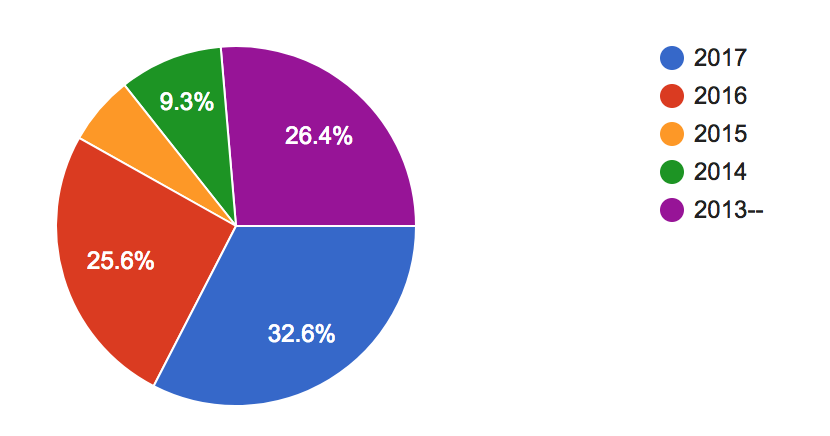
\includegraphics{pics/angkatan}
		\caption{Responden berdasarkan angkatan}
		\centering
	\end{figure}
	Responden kuisoner ini memiliki persebaran pernah mempelajari pemrograman sebelum mengikuti mata kuliah Dasar Dasar Pemograman. Responden yang pernah mempelajari pemrograman sebelum mengikuti kuliah Dasar Dasar Pemograman sebanyak 62 responden (48,8\%) dan yang belum pernah mempelajari pemrograman sebelum mengikuti kuliah Dasar Dasar Pemograman sebanyak 66 (51,2\%). Informasi ini terangkum dalam Gambar 4.2 berikut.
	\begin{figure}
		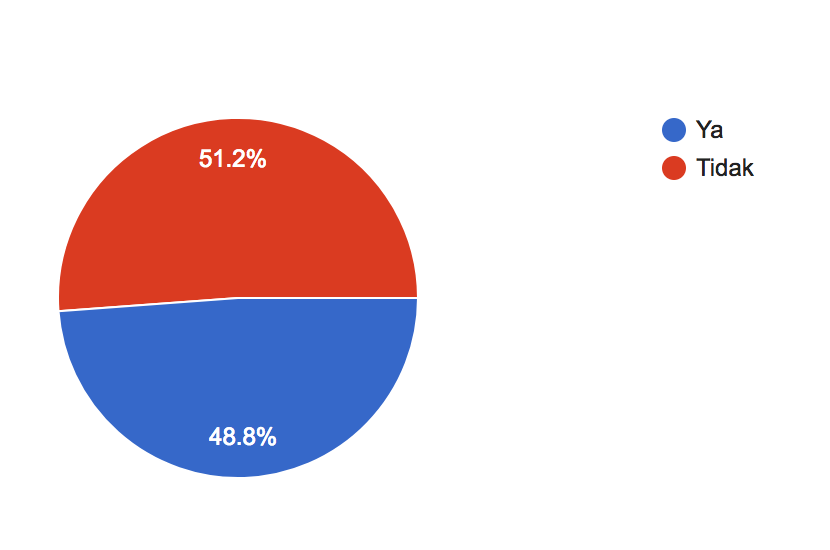
\includegraphics[width=\linewidth]{pics/pernah-ikut-ddp-sebelum}
		\caption{Responden pernah mempelajari DDP sebelumnya}
		\centering
	\end{figure}
	Dari yang telah mempelajari sebelumnya, sebanyak 42 responden mempelajarinya saat SMA, 15 responden saat SMP, dan 2 responden mempelajarinya antara SMA dan kuliah. Informasi ini terangkum dalam Gambar 4.3 berikut.
	\begin{figure}
		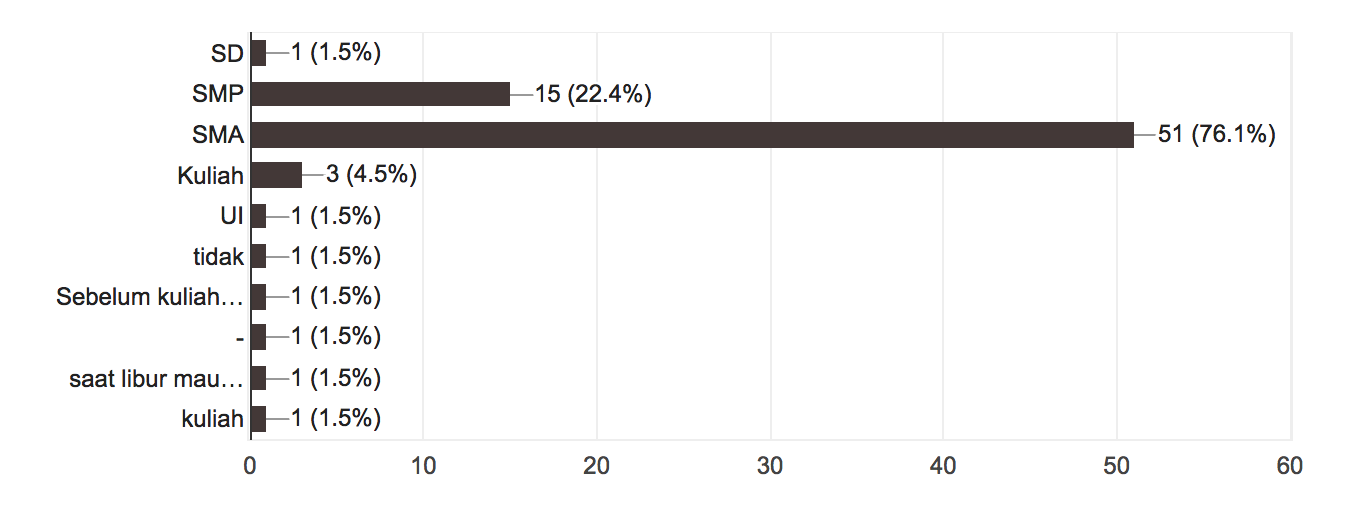
\includegraphics[width=\linewidth]{pics/kapan-pernah-belajarnya}
		\caption{Waktu mempelajari DDP}
		\centering
	\end{figure}
	Responden yang menganggap pemrograman merupakan minat mereka sebanyak 42 responden, yang mengatakan pemrograman bukan merupakan minat mereka sebanyak 14 responden, dan sebanyak 72 responden ragu untuk mengatakan pemrograman merupakan minat mereka. Informasi ini dapat dilihat pada Gambar 4.4 berikut.
	\begin{figure}
		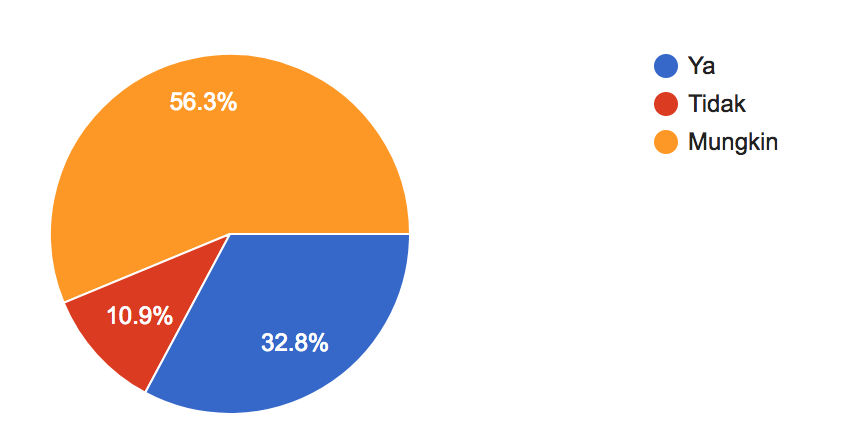
\includegraphics[width=\linewidth]{pics/passion-pemograman}
		\caption{Persebaran minat responden terhadap pemrograman}
		\centering
	\end{figure}
	Responden mengalokasikan waktu selama 3 - 5 jam dalam satu pekan untuk belajar pemrograman sebanyak 43 orang (33.6\%), 5 - 7 jam dalam satu pekan sebanyak 40 orang (31,3\%),  7 - 10 jam dalam satu pekan sebanyak 20 orang (15,6\%), kurang dari 3 jam dalam satu pekan sebanyak 17 orang (13,3\%), dan lebih dari 10 jam dalam satu pekan sebanyak 8 orang (6,3\%). Informasi ini terangkum dalam Gambar 4.5.
	\begin{figure}
		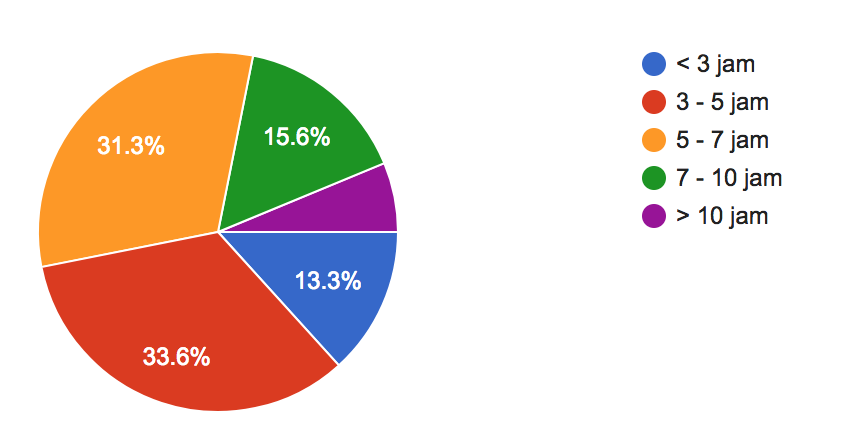
\includegraphics[width=\linewidth]{pics/lama-belajar}
		\caption{Lama belajar responden dalam satu pekan}
		\centering
	\end{figure}
	Responden diminta untuk memberikan nilai kepada dirinya sendiri sejauh mana mereka memahami pemrograman itu dengan nilai 1 - 10. Sebanyak 43 orang memberikan nilai 7, 26 orang memberikan nilai 8, 24 orang memberikan nilai 6, 11 orang memberikan nilai 5, 7 orang memberikan nilai 10, 6 orang memberikan nilai 4, 5 orang memberikan nilai 3, 4 orang memberikan nilai 2, dan 1 orang memberikan nilai 9 dan 1. Infromasi ini dapat dilihat pada Gambar 4.6.
	\begin{figure}
		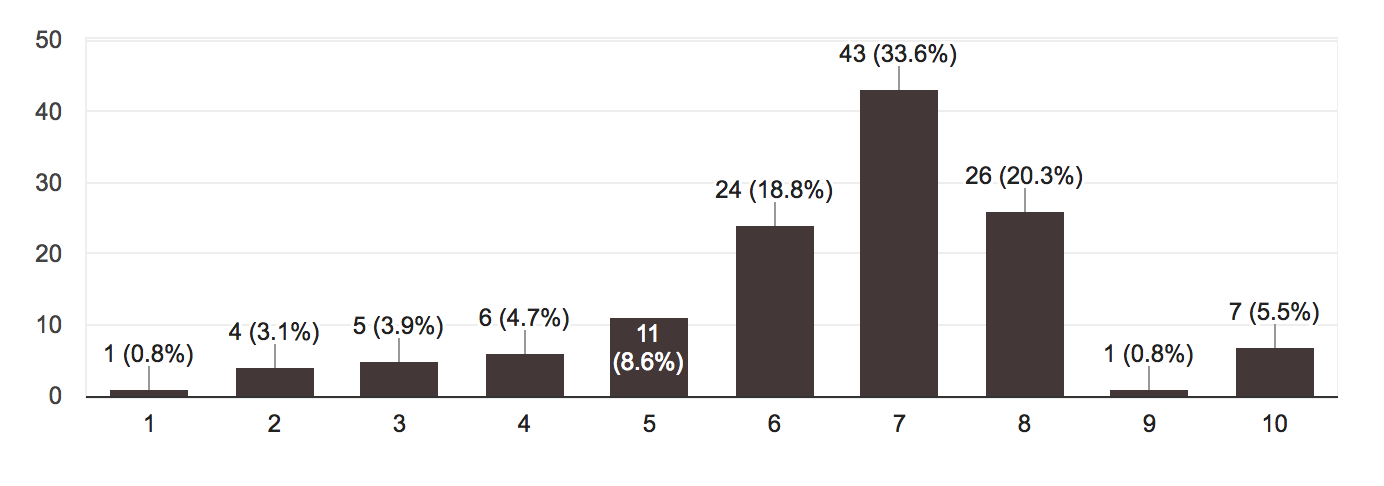
\includegraphics[width=\linewidth]{pics/nilai-pemograman}
		\caption{Nilai responden terhadap dirinya sendiri mengenai pemrograman}
		\centering
	\end{figure}
	Responden yang masuk dalam kategori sudah pernah mengambil DDP sebelumnya, terdapat 10 responden (9,6\%) yang mengulang mata kuliah DDP. dan 94 responden (90,4\%) yang tidak mengulang mata kuliah DDP. Informasi ini terdapat dalam Gambar 4.7 berikut.
	\begin{figure}
		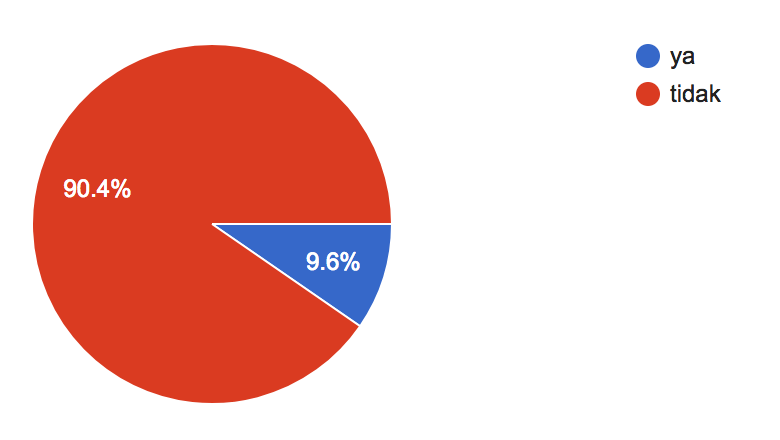
\includegraphics[width=\linewidth]{pics/mengulang-ddp}
		\caption{Persebaran responden yang mengulang}
		\centering
	\end{figure}
	Sebanyak 101 responden (78,9\%) mengatakan bahwa mereka sangat suka diberikan contoh langsung dari materi yang sedang diajarkan, 24 responden (18,8\%) suka diberikan contoh langsung, dan 3 (2,3\%) biasa saja dijika diberikan contoh langsung. informasi ini terlihat dalam Gambar 4.8.
	\begin{figure}
		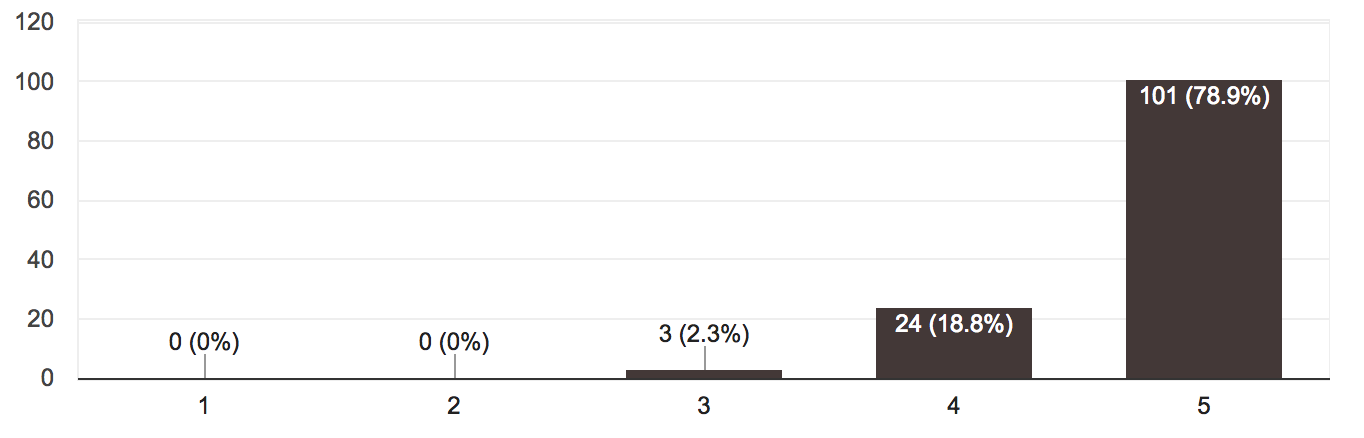
\includegraphics[width=\linewidth]{pics/contoh-langsung}
		\caption{Tingkat setuju terhadap pernyataan suka nya responden diberikan contoh langsung saat diberikan materi DDP}
		\centering
	\end{figure}
	Diberikan pernyataan bahwa responden memerlukan waktu diluar kelas untuk mempelajari lagi materi DDP. 50 responden sangat setuju, 43 setuju, 25 biasa saja, 7 tidak setuju, 3 sangat tidak setuju. Infromasi ini terkandung dalam Gambar 4.9.
	\begin{figure}
		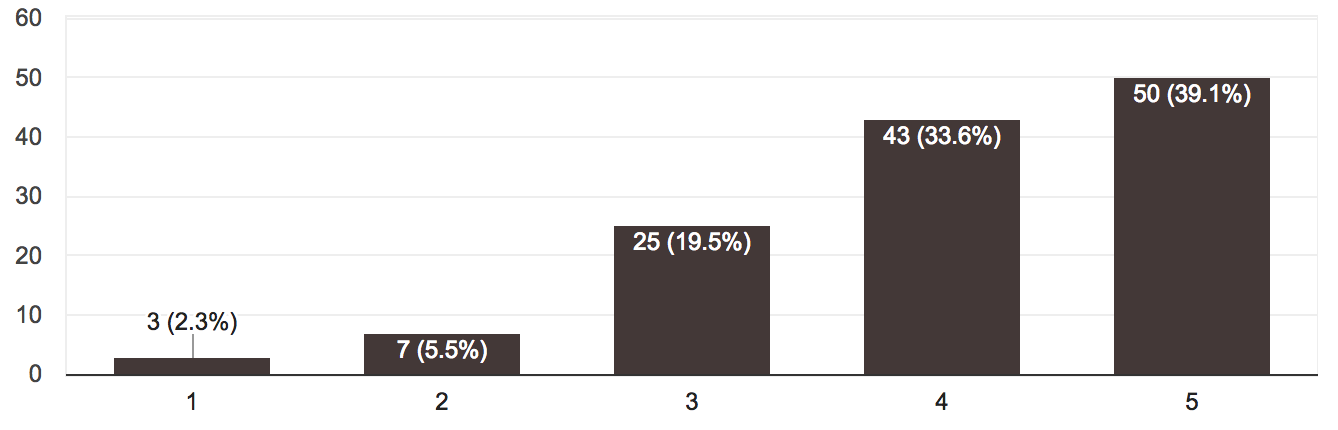
\includegraphics[width=\linewidth]{pics/perlu-waktu-luar-kelas}
		\caption{Tingkat setuju terhadap pernyataan memerlukan waktu diluar kelas untuk memahami materi DDP}
		\centering
	\end{figure}
	Sebanyak 100 responden (78,1\%)suka bermain game, dan 28 responden (21,9\%) tidak suka bermain game. Informasi ini terdapat pada Gambar 4.10 berikut.
	\begin{figure}
		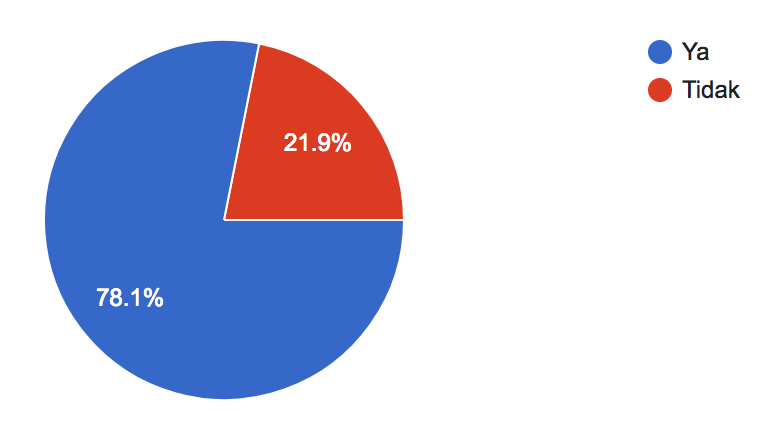
\includegraphics[width=\linewidth]{pics/suka-bermain-game}
		\caption{Alur tahapan penelitian}
		\centering
	\end{figure}
	Waktu yang dihabiskan oleh 54 responden (42,2\%) kurang dari 3 jam dalam satu sepekan, 29 responden (22,7\%) 3 - 5 jam dalam satu pekan, 20 responden (15,6\%) 5 - 7 jam dalam satu pekan, 17 responden (13,3\%) lebih dari 10 jam dalam satu pekan, 8 responden (6,3\%) 7 - 10 jam dalam satu pekan. Data ini tergambarkan dalam Gambar 4.11 berikut.
	\begin{figure}
		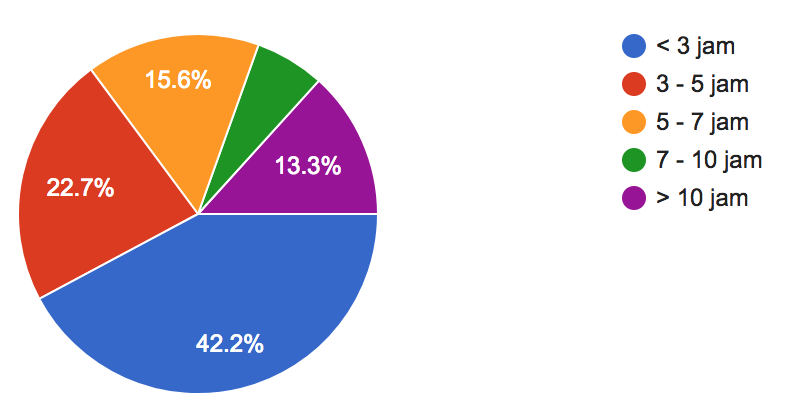
\includegraphics[width=\linewidth]{pics/waktu-bermain-game}
		\caption{Alur tahapan penelitian}
		\centering
	\end{figure}
	Responden yang lebih suka bermain \textit{game} jika dibandingkan dengan mempelajari pemrograman sebanyak 67 responden (52,3\%), 48 responden (37,5\%) ragu - ragu atau sama saja, dan 13 responden (10,2\%) mengatakan lebih suka mempelajari pemrograman dari bermain \textit{game}. Informasi ini terdapat pada Gambar 4.12 berikut.
	\begin{figure}
		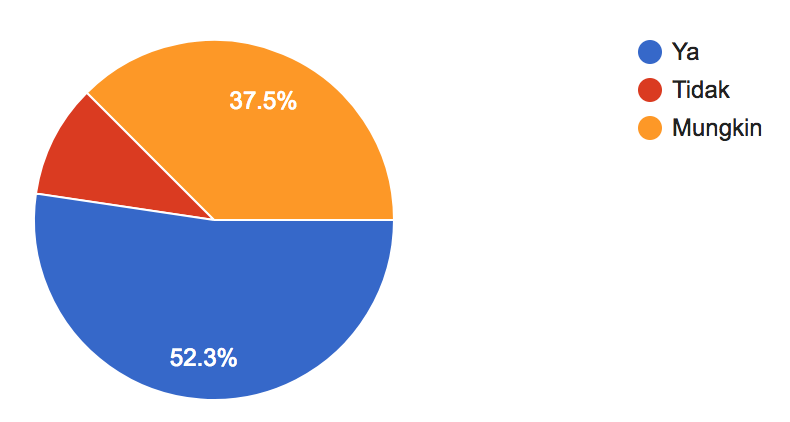
\includegraphics[width=\linewidth]{pics/lebih-senang-bermain-game}
		\caption{Persebaran lebih senang bermain \textit{game} dari belajar pemrograman}
		\centering
	\end{figure}
%
%	\begin{figure}
%		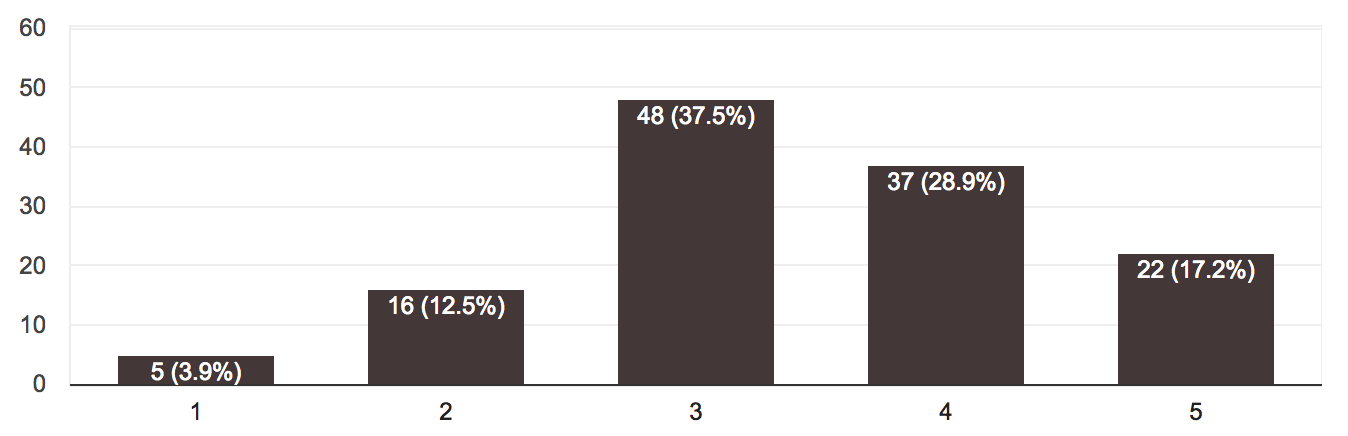
\includegraphics[width=\linewidth]{pics/menggali-lebih-dalam-sendiri}
%		\caption{Alur tahapan penelitian}
%		\centering
%	\end{figure}
%	\begin{figure}
%		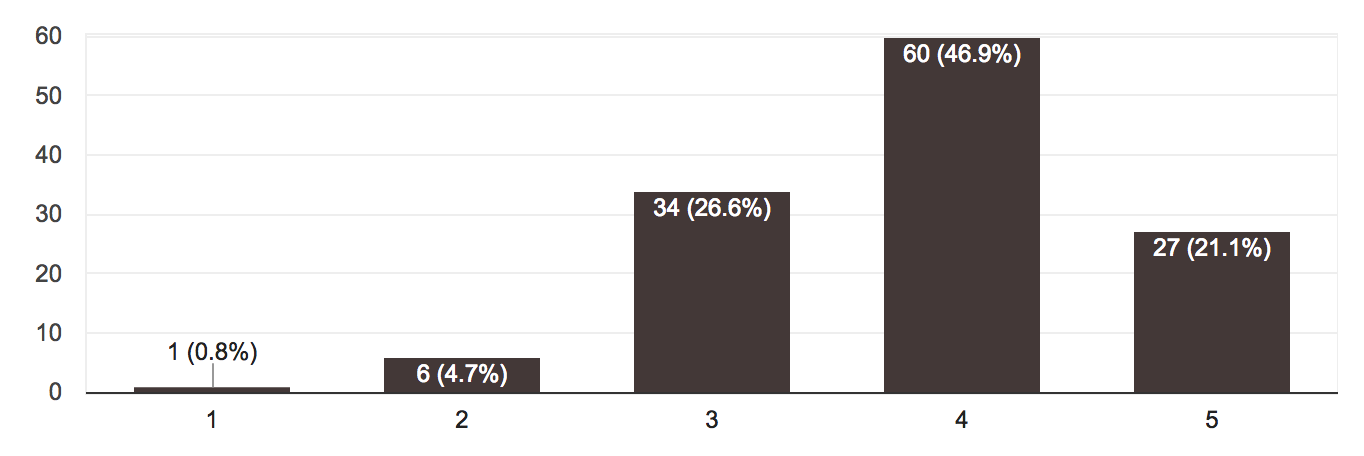
\includegraphics[width=\linewidth]{pics/menikmati-cara-belajar-sekarang}
%		\caption{Alur tahapan penelitian}
%		\centering
%	\end{figure}
%	\begin{figure}
%		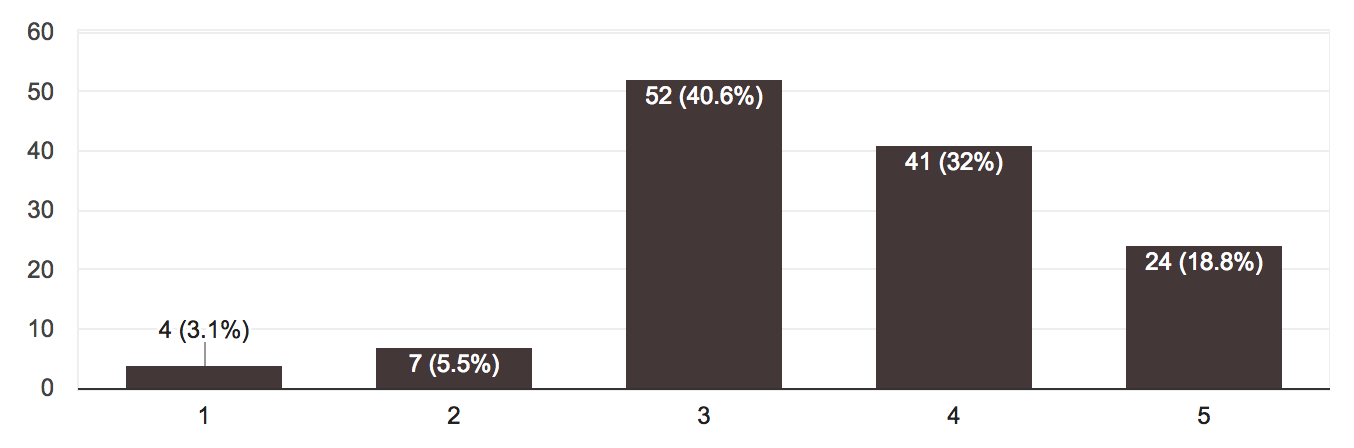
\includegraphics[width=\linewidth]{pics/mudah-memahami}
%		\caption{Alur tahapan penelitian}
%		\centering
%	\end{figure}
%	\begin{figure}
%		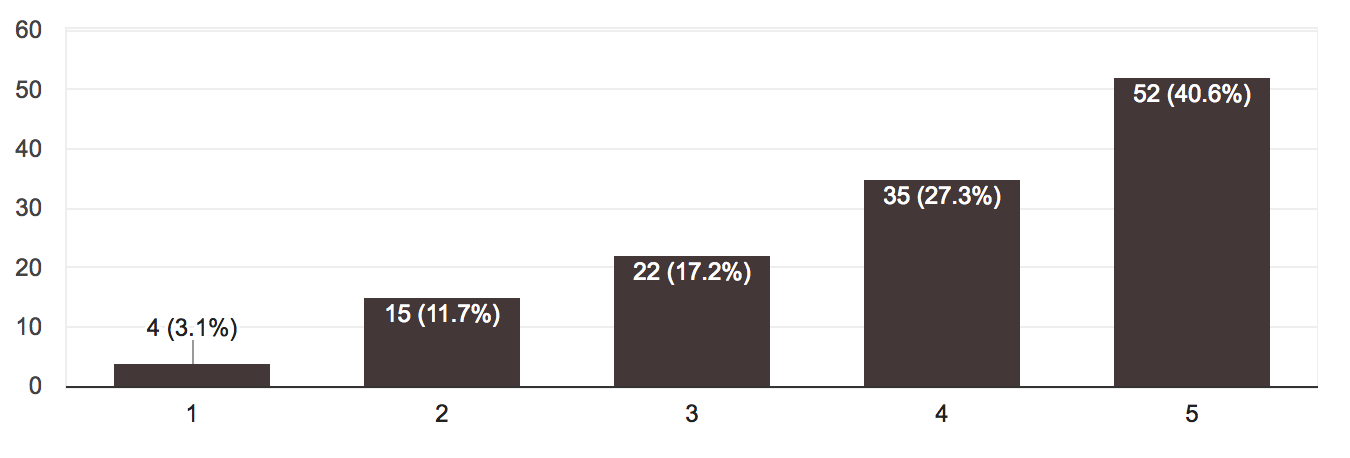
\includegraphics[width=\linewidth]{pics/slide-show-x-buku}
%		\caption{Alur tahapan penelitian}
%		\centering
%	\end{figure}
%	\begin{figure}
%		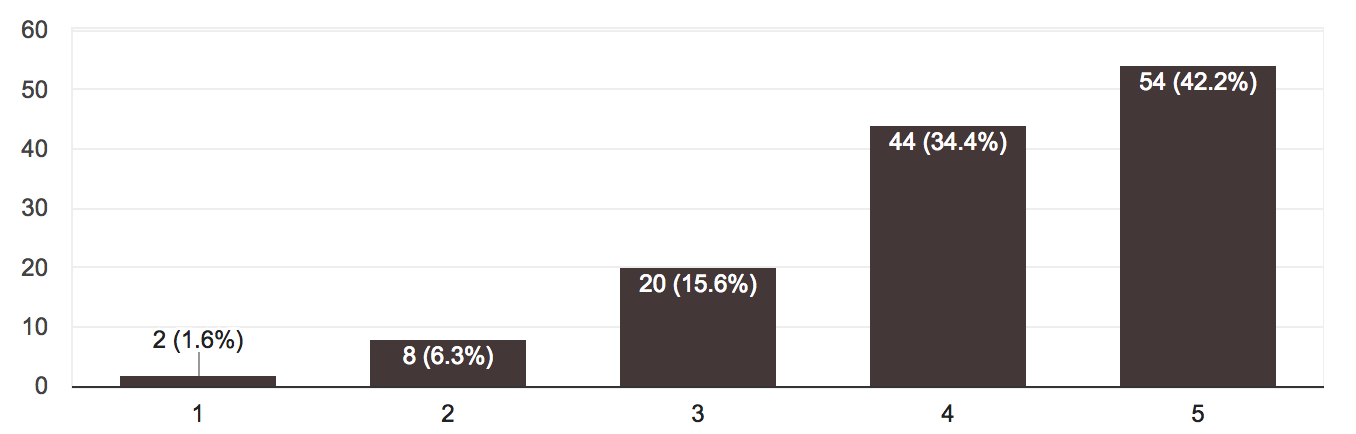
\includegraphics[width=\linewidth]{pics/tidak-suka-teori-saja}
%		\caption{Alur tahapan penelitian}
%		\centering
%	\end{figure}
% this should data kualitatif
Pada bagian \textit{open-ended} pada kuisoner, dikelompokan sesuai dengan yang telah dijelaskan pada bab 3.2.3.
\begin{table}
	\centering
	\caption{Pengertian pemrograman}
	\label{tab:tab1}
	\begin{tabular}{| c | c | c |}
		\hline
		Kode & Konten & n \\
		\hline
		PP1 & \multicolumn{1}{p{10cm}|}{membuat program} & 37 \\ \hline
		PP2 & \multicolumn{1}{p{10cm}|}{Proses dimana manusia membahasakan suatu kumpulan instruksi agar dapat dimengerti dan dijalankan oleh komputer} & 34 \\ \hline
		PP3 & \multicolumn{1}{p{10cm}|}{\textit{Problem solving} atau penyelesaian sebuah masalah} & 27 \\
		\hline
		PP4 & \multicolumn{1}{p{10cm}|}{Tidak dapat mengartikan pemrograman} & 15 \\ \hline
		PP5 & \multicolumn{1}{p{10cm}|}{Serangkaian kode untuk mencapai tujuan tertentu} & 13 \\ \hline
		PP6 & \multicolumn{1}{p{10cm}|}{Pola pikir} & 1 \\ \hline
		PP7 & \multicolumn{1}{p{10cm}|}{Mempelajari bahasa pemrograman} & 1 \\ \hline
		PP8 & \multicolumn{1}{p{10cm}|}{Jembatan komunikasi antara manusia dengan teknologi} & 1 \\ \hline
	\end{tabular}
\end{table}

\section{Mendefinisikan Persona dan Spesifikasi Sistem}
Pada subbab ini akan diberikan hasil dari hasil survei dan demografi yang dipaparkan pada subbab 4.1. Setelah didapatkan hasil maka terbentuk persona yang menjadi gambaran umum dari responden dan juga spesifikasi sistem yang akan dibuat dari estetika, mekanik, teknologi dan naratifnya.

	\subsection{Persona}
	Persona ditentukan berdasarkan demografi responden terbanyak pada kuesioner adalah mahasiswa yang sudah menerima pelajaran pemrograman dari sebelum kuliah dan persona kedua adalah belum menerima pelajaran pemrograman dari sebelum kuliah. Berikut merupakan gambaran kedua persona tersebut.
	\begin{figure}
		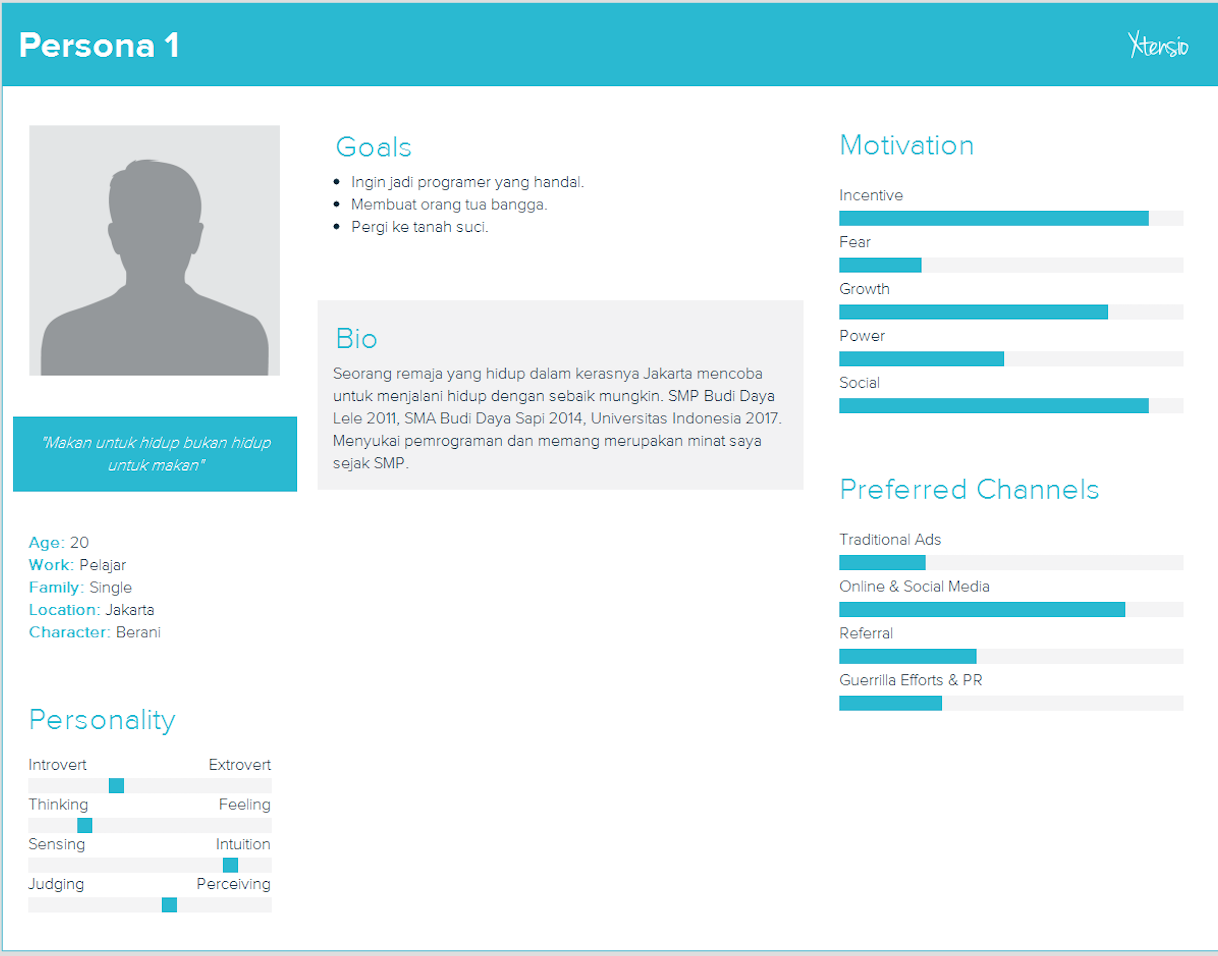
\includegraphics[width=\linewidth]{pics/pesona1}
		\caption{Persona 1}
		\centering
	\end{figure}
	\begin{figure}
		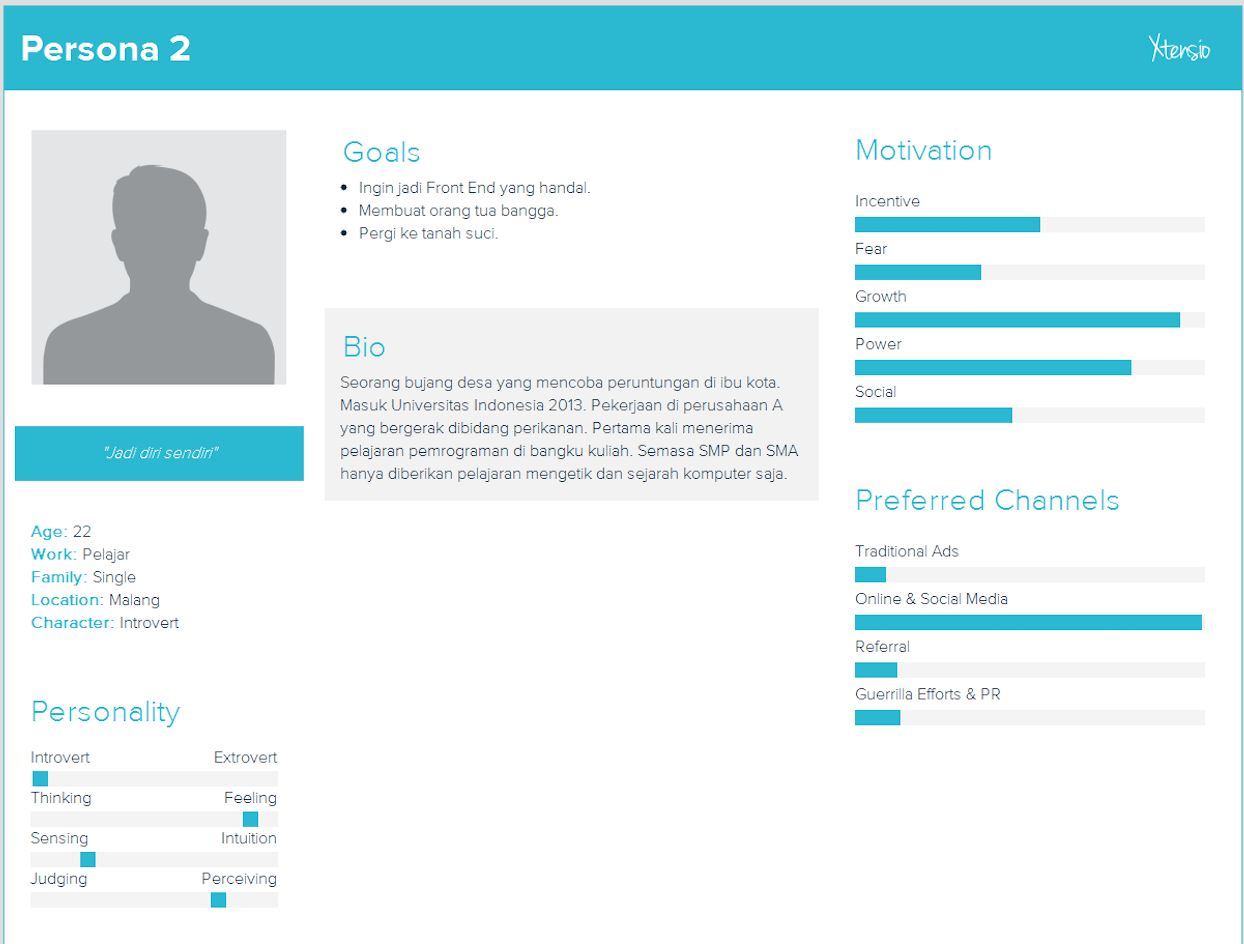
\includegraphics[width=\linewidth]{pics/pesona2}
		\caption{Persona 2}
		\centering
	\end{figure}
	\subsection{Spesifikasi Sistem}
		\subsubsection{Estetika}
		\subsubsection{Mekanik}
		\subsubsection{Teknologi}
		Teknologi yang digunakan adalah Unity sebagai media pembuatan sistem.
		\subsubsection{Naratif}

	


